\chapter{Introduction}

\section{Abstract}
\begin{figure}[htp]
\begin{center}
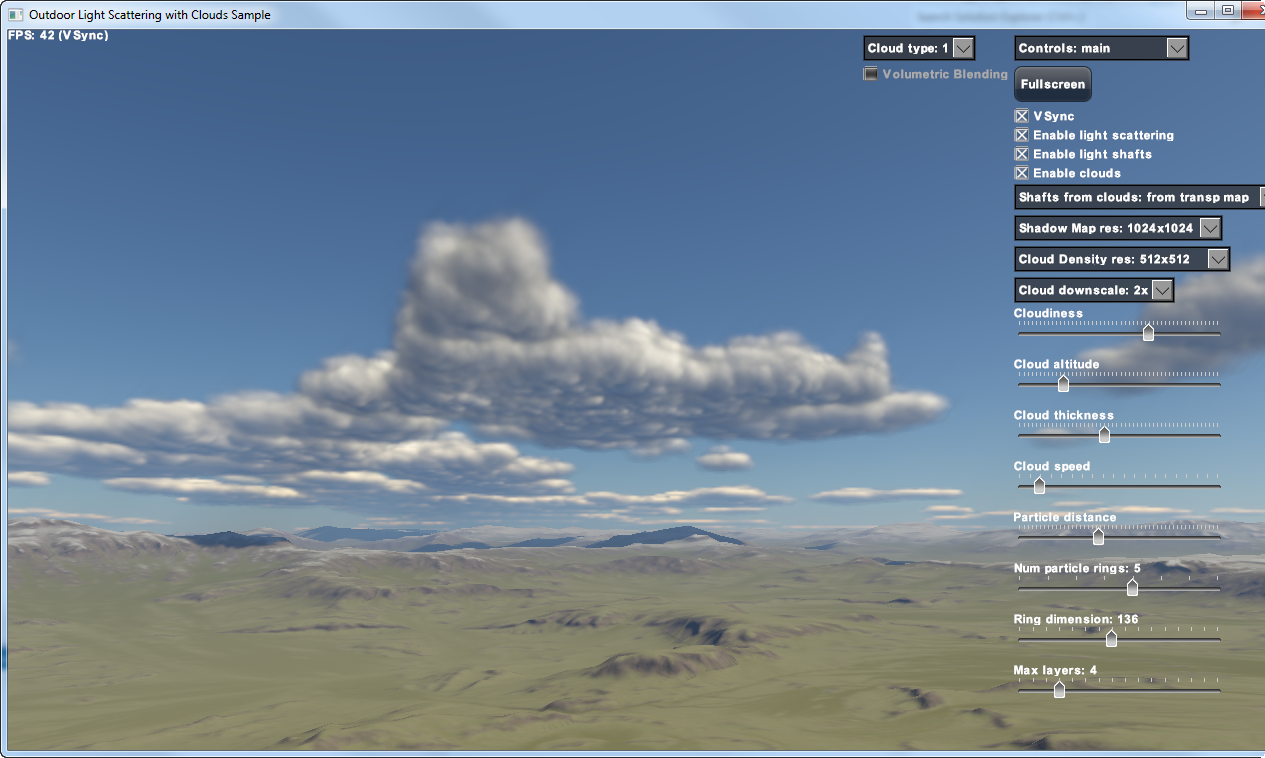
\includegraphics[scale=0.4]{images/overview.png}
\caption{Overview}
\label{f0}
\end{center}
\end{figure}

In the paper, the author introduced a new method for rendering realistic cumulus clouds in real time. The basic steps include:
\begin{enumerate}
\item Pre-computing optical depth.
\item Pre-computing scattering.
\item Generating a real-time lighting model from the above two steps.
\item Volume-aware blending the particles.
\item Controlling the level of details.
\end{enumerate}
He also explained the mathematical background to solve the problem. The paper is interesting, but hard to understand. I'm writing this review to make the author's ideas easier to be understood. And I will also supplement to some uncertain explanation from the author with my personal thoughts. Finally, I'll include a conclusion section in the end of each chapter to elaborate my opinions to the author's approach.